\documentclass{article}
\usepackage{tikz}
\usepackage{geometry}
\usepackage[dvipsnames]{xcolor}
\pagestyle{empty}
\usepackage{luatexja}
\renewcommand{\kanjifamilydefault}{\gtdefault}
\renewcommand{\familydefault}{\sfdefault}

\newcommand{\docpaperwidth}{8cm}
\newcommand{\docpaperheight}{3cm}

\geometry{
  papersize={\docpaperwidth,\docpaperheight},
  margin=0.5cm,
  ignoreall=true
}
\usetikzlibrary{backgrounds}
\usetikzlibrary{shapes.geometric}
\usetikzlibrary{calc}

\setlength{\parindent}{0cm}

% grid cell width
\newcommand{\grdclw}{1cm}

% grid cell half width
\newcommand{\grdclwh}{0.5cm}
% grid cell quater width 
\newcommand{\grdclwq}{0.25cm}

% grid cell height
\newcommand{\grdclh}{0.5cm}
% grid cell half height
\newcommand{\grdclhh}{0.25cm}

%baseline offset from center for horizontal text
\newcommand{\bsloffseth}{-0.1cm}

%baseline offset from cenete for vertical text
\newcommand{\bsloffsetv}{0.1cm} 

% grid column x position a
\newcommand{\grdclxa}{0.2cm}
% grid column x position b
\newcommand{\grdclxb}{\grdclxa + \grdclwh}
% grid column x position c
\newcommand{\grdclxc}{\grdclxb + \grdclwh}
% grid column x position d
\newcommand{\grdclxd}{\grdclxc + \grdclw}
% grid column x position e
\newcommand{\grdclxe}{\grdclxd + \grdclw}
% grid column x position f
\newcommand{\grdclxf}{\grdclxe + \grdclw}
% grid column x position g
\newcommand{\grdclxg}{\grdclxf + \grdclw}
% grid column x position h
\newcommand{\grdclxh}{\grdclxg + \grdclw}
% grid column x position i 
\newcommand{\grdclxi}{\grdclxh + \grdclw}

% grid node x position a
\newcommand{\grdnxa}{\grdclxa + \grdclwq + \bsloffsetv}

% grid node x position b
\newcommand{\grdnxb}{\grdclxb + \grdclwq + \bsloffsetv}

% grid node x position c
\newcommand{\grdnxc}{\grdclxc + \grdclwh}

% grid node x position d
\newcommand{\grdnxd}{\grdclxd + \grdclwh}

% grid node x position e
\newcommand{\grdnxe}{\grdclxe + \grdclwh}

% grid node x position f
\newcommand{\grdnxf}{\grdclxf + \grdclwh}

% grid node x position g
\newcommand{\grdnxg}{\grdclxg + \grdclwh}

% grid node x position h
\newcommand{\grdnxh}{\grdclxh + \grdclwh}


% grid left offset
\newcommand{\grdosl}{0.03cm}

% grid right offset
\newcommand{\grdosr}{-0.03cm}

% grid bottom offset
\newcommand{\grdosb}{0.03cm}

% grid top offset
\newcommand{\grdost}{-0.03cm}

% grid column y position a
\newcommand{\grdclya}{0}

% grid column y position b
\newcommand{\grdclyb}{\grdclya + \grdclh}
% grid column y position c
\newcommand{\grdclyc}{\grdclyb + \grdclh}
% grid column y position d
\newcommand{\grdclyd}{\grdclyc + \grdclh}
% grid column y position e
\newcommand{\grdclye}{\grdclyd + \grdclh}
% grid node y position a
\newcommand{\grdnya}{\grdclya + \grdclhh + \bsloffseth}
% grid node y position b
\newcommand{\grdnyb}{\grdclyb + \grdclhh + \bsloffseth}
% grid node y position c
\newcommand{\grdnyc}{\grdclyc + \grdclhh + \bsloffseth}
 
% (a, a) - (b, e) rectangle
\newcommand{\rectaabe}{\pgfpathrectanglecorners
  {\pgfpoint{\grdclxa + \grdosl}{\grdclya + \grdosb}}
  {\pgfpoint{\grdclxb + \grdosr}{\grdclye + \grdost}}}

% (b, a) - (c, e) rectangle
\newcommand{\rectbace}{\pgfpathrectanglecorners
  {\pgfpoint{\grdclxb + \grdosl}{\grdclya + \grdosb}}
  {\pgfpoint{\grdclxc + \grdosr}{\grdclye + \grdost}}}

% (c, a) - (d, b) rectangle
\newcommand{\rectcadb}{\pgfpathrectanglecorners
  {\pgfpoint{\grdclxc + \grdosl}{\grdclya + \grdosb}}
  {\pgfpoint{\grdclxd + \grdosr}{\grdclyb + \grdost}}}

% (d, a) - (e, b) rectangle
\newcommand{\rectdaeb}{
  \pgfpathrectanglecorners
    {\pgfpoint{\grdclxd + \grdosl}{\grdclya + \grdosb}}
    {\pgfpoint{\grdclxe + \grdosr}{\grdclyb + \grdost}}} 

% (e, a) - (f, b) rectangle
\newcommand{\recteafb}{
  \pgfpathrectanglecorners
    {\pgfpoint{\grdclxe + \grdosl}{\grdclya + \grdosb}}
    {\pgfpoint{\grdclxf + \grdosr}{\grdclyb + \grdost}}}

% (f, a) - (g, b) rectangle
\newcommand{\rectfagb}{
  \pgfpathrectanglecorners
    {\pgfpoint{\grdclxf + \grdosl}{\grdclya + \grdosb}}
    {\pgfpoint{\grdclxg + \grdosr}{\grdclyb + \grdost}}} 

% (g, a) - (h, b) rectangle
\newcommand{\rectgahb}{
  \pgfpathrectanglecorners
    {\pgfpoint{\grdclxg + \grdosl}{\grdclya + \grdosb}}
    {\pgfpoint{\grdclxh + \grdosr}{\grdclyb + \grdost}}} 

% (h, a) - (i, b) rectangle
\newcommand{\recthaib}{
  \pgfpathrectanglecorners
    {\pgfpoint{\grdclxh + \grdosl}{\grdclya + \grdosb}}
    {\pgfpoint{\grdclxi + \grdosr}{\grdclyb + \grdost}}} 

% (c, b) - (i, c) rectangle
\newcommand{\rectcbic}{
  \pgfpathrectanglecorners
    {\pgfpoint{\grdclxc + \grdosl}{\grdclyb + \grdosb}}
    {\pgfpoint{\grdclxi + \grdosr}{\grdclyc + \grdost}}} 

% (c, c) - (i, e) rectangle
\newcommand{\rectccie}{
  \pgfpathrectanglecorners
    {\pgfpoint{\grdclxc + \grdosl}{\grdclyc + \grdosb}}
    {\pgfpoint{\grdclxi + \grdosr}{\grdclye + \grdost}}}


\begin{document}
  \center
  % hw firm uefi stack
  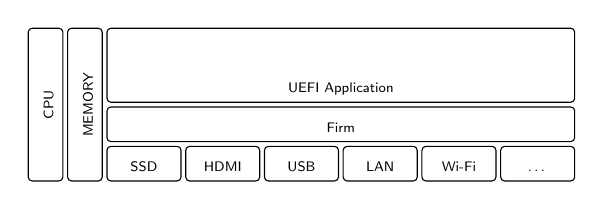
\begin{tikzpicture}[anchor=base,font=\tiny]

    \node at ($(\grdnxa, 0)
      + 0.5*(0, \grdclya + \grdclyc + \grdclw)$) [rotate=90] {CPU};
    \node at ($(\grdnxb, 0)
      + 0.5*(0, \grdclya + \grdclyc + \grdclw)$) [rotate=90] {MEMORY};

    \node at (\grdnxc, \grdnya) {SSD};
    \node at (\grdnxd, \grdnya) {HDMI};
    \node at (\grdnxe, \grdnya) {USB};
    \node at (\grdnxf, \grdnya) {LAN};
    \node at (\grdnxg, \grdnya) {Wi-Fi};
    \node at (\grdnxh, \grdnya) {\ldots};
    \node at ($(0.5*(\grdclxc + \grdclxh + \grdclw, 0)
      + (0, \grdnyb)$) {Firm};
    \node at ($(0.5*(\grdclxc + \grdclxh + \grdclw, 0)
      + (0, \grdnyc)$) {UEFI Application};
    \begin{scope}[on background layer]
      \pgfsetcornersarced{\pgfpoint{0.05cm}{0.05cm}}
      \rectaabe
      \pgfusepath{stroke}
      \rectbace
      \pgfusepath{stroke}
      \rectcadb
      \pgfusepath{stroke}
      \rectdaeb
      \pgfusepath{stroke}
      \recteafb
      \pgfusepath{stroke}
      \rectfagb
      \pgfusepath{stroke}
      \rectgahb
      \pgfusepath{stroke}
      \recthaib
      \pgfusepath{stroke}
      \rectcbic
      \pgfusepath{stroke}
      \rectccie
      \pgfusepath{stroke}
    \end{scope}
  \end{tikzpicture}
  \newpage
  % hw firm  stack
  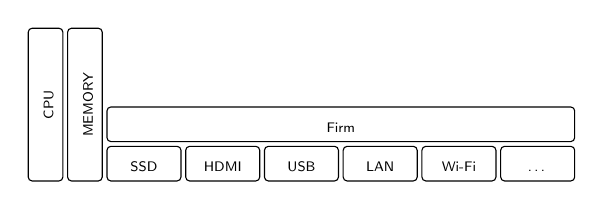
\begin{tikzpicture}[anchor=base,font=\tiny]
    \node at ($(\grdnxa, 0)
      + 0.5*(0, \grdclya + \grdclyc + \grdclw)$) [rotate=90] {CPU};
    \node at ($(\grdnxb, 0)
      + 0.5*(0, \grdclya + \grdclyc + \grdclw)$) [rotate=90] {MEMORY};

    \node at (\grdnxc, \grdnya) {SSD};
    \node at (\grdnxd, \grdnya) {HDMI};
    \node at (\grdnxe, \grdnya) {USB};
    \node at (\grdnxf, \grdnya) {LAN};
    \node at (\grdnxg, \grdnya) {Wi-Fi};
    \node at (\grdnxh, \grdnya) {\ldots};
    \node at ($(0.5*(\grdclxc + \grdclxh + \grdclw, 0)
      + (0, \grdnyb)$) {Firm};

    \begin{scope}[on background layer]
      \pgfsetcornersarced{\pgfpoint{0.05cm}{0.05cm}}
      \rectaabe
      \pgfusepath{stroke}
      \rectbace
      \pgfusepath{stroke}
      \rectcadb
      \pgfusepath{stroke}
      \rectdaeb
      \pgfusepath{stroke}
      \recteafb
      \pgfusepath{stroke}
      \rectfagb
      \pgfusepath{stroke}
      \rectgahb
      \pgfusepath{stroke}
      \recthaib
      \pgfusepath{stroke}
      \rectcbic
      \pgfusepath{stroke}
    \end{scope}
  \end{tikzpicture}
  \newpage
  % hw firm stack power on 1
  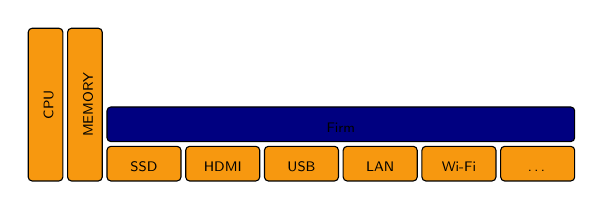
\begin{tikzpicture}[anchor=base,font=\tiny]
    \node at ($(\grdnxa, 0)
      + 0.5*(0, \grdclya + \grdclyc + \grdclw)$) [rotate=90] {CPU};
    \node at ($(\grdnxb, 0)
      + 0.5*(0, \grdclya + \grdclyc + \grdclw)$) [rotate=90] {MEMORY};

    \node at (\grdnxc, \grdnya) {SSD};
    \node at (\grdnxd, \grdnya) {HDMI};
    \node at (\grdnxe, \grdnya) {USB};
    \node at (\grdnxf, \grdnya) {LAN};
    \node at (\grdnxg, \grdnya) {Wi-Fi};
    \node at (\grdnxh, \grdnya) {\ldots};
    \node at ($(0.5*(\grdclxc + \grdclxh + \grdclw, 0)
      + (0, \grdnyb)$) {Firm};

    \begin{scope}[on background layer]
      \pgfsetcornersarced{\pgfpoint{0.05cm}{0.05cm}}
      \color{YellowOrange}
      \rectaabe
      \pgfusepath{fill}
      \rectbace
      \pgfusepath{fill}
      \rectcadb
      \pgfusepath{fill}
      \rectdaeb
      \pgfusepath{fill}
      \recteafb
      \pgfusepath{fill}
      \rectfagb
      \pgfusepath{fill}
      \rectgahb
      \pgfusepath{fill}
      \recthaib
      \pgfusepath{fill}
      \color{NavyBlue} 
      \rectcbic
      \pgfusepath{fill}
      \color{black}
      \rectaabe
      \pgfusepath{stroke}
      \rectbace
      \pgfusepath{stroke}
      \rectcadb
      \pgfusepath{stroke}
      \rectdaeb
      \pgfusepath{stroke}
      \recteafb
      \pgfusepath{stroke}
      \rectfagb
      \pgfusepath{stroke}
      \rectgahb
      \pgfusepath{stroke}
      \recthaib
      \pgfusepath{stroke}
      \rectcbic
      \pgfusepath{stroke}
    \end{scope}
  \end{tikzpicture}
  \newpage
  % hw firm stack ipxe load from usb
  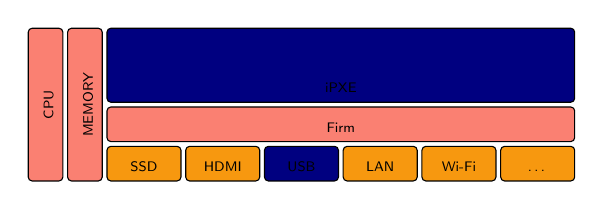
\begin{tikzpicture}[anchor=base,font=\tiny]
    \node at ($(\grdnxa, 0)
      + 0.5*(0, \grdclya + \grdclyc + \grdclw)$) [rotate=90] {CPU};
    \node at ($(\grdnxb, 0)
      + 0.5*(0, \grdclya + \grdclyc + \grdclw)$) [rotate=90] {MEMORY};

    \node at (\grdnxc, \grdnya) {SSD};
    \node at (\grdnxd, \grdnya) {HDMI};
    \node at (\grdnxe, \grdnya) {USB};
    \node at (\grdnxf, \grdnya) {LAN};
    \node at (\grdnxg, \grdnya) {Wi-Fi};
    \node at (\grdnxh, \grdnya) {\ldots};
    \node at ($(0.5*(\grdclxc + \grdclxh + \grdclw, 0)
      + (0, \grdnyb)$) {Firm};
    \node at ($(0.5*(\grdclxc + \grdclxh + \grdclw, 0)
      + (0, \grdnyc)$) {iPXE};
 
    \begin{scope}[on background layer]
      \pgfsetcornersarced{\pgfpoint{0.05cm}{0.05cm}}
      \color{Salmon}
      \rectaabe
      \pgfusepath{fill}
      \rectbace
      \pgfusepath{fill}

      \color{YellowOrange}
      \rectcadb
      \pgfusepath{fill}
      \rectdaeb
      \pgfusepath{fill}
      {
        \color{NavyBlue}
        \recteafb
        \pgfusepath{fill}
      }
      \rectfagb
      \pgfusepath{fill}
      \rectgahb
      \pgfusepath{fill}
      \recthaib
      \pgfusepath{fill}
      \color{Salmon}
      \rectcbic
      \pgfusepath{fill}
      \color{NavyBlue}
      \rectccie
      \pgfusepath{fill}

      \color{black}
      \rectaabe
      \pgfusepath{stroke}
      \rectbace
      \pgfusepath{stroke}
      \rectcadb
      \pgfusepath{stroke}
      \rectdaeb
      \pgfusepath{stroke}
      \recteafb
      \pgfusepath{stroke}
      \rectfagb
      \pgfusepath{stroke}
      \rectgahb
      \pgfusepath{stroke}
      \recthaib
      \pgfusepath{stroke}
      \rectcbic
      \pgfusepath{stroke}
      \rectccie
      \pgfusepath{stroke}
    \end{scope}
  \end{tikzpicture}
  \newpage
  % hw firm stack installer linux loaded by iPXE
  \begin{tikzpicture}[anchor=base,font=\tiny]
    \node at ($(\grdnxa, 0)
      + 0.5*(0, \grdclya + \grdclyc + \grdclw)$) [rotate=90] {CPU};
    \node at ($(\grdnxb, 0)
      + 0.5*(0, \grdclya + \grdclyc + \grdclw)$) [rotate=90] {MEMORY};

    \node at (\grdnxc, \grdnya) {SSD};
    \node at (\grdnxd, \grdnya) {HDMI};
    \node at (\grdnxe, \grdnya) {USB};
    \node at (\grdnxf, \grdnya) {LAN};
    \node at (\grdnxg, \grdnya) {Wi-Fi};
    \node at (\grdnxh, \grdnya) {\ldots};
    \node at ($(0.5*(\grdclxc + \grdclxh + \grdclw, 0)
      + (0, \grdnyb)$) {Firm};
    \node at ($(0.5*(\grdclxc + \grdclxh + \grdclw, 0)
      + (0, \grdnyc)$) {インストーラLinux iPXEによりロード};
 
    \begin{scope}[on background layer]
      \pgfsetcornersarced{\pgfpoint{0.05cm}{0.05cm}}
      \color{Salmon}
      \rectaabe
      \pgfusepath{fill}
      \rectbace
      \pgfusepath{fill}

      \color{YellowOrange}
      \rectcadb
      \pgfusepath{fill}
      \rectdaeb
      \pgfusepath{fill}
      \recteafb
      \pgfusepath{fill}
      {
        \color{NavyBlue}
        \rectfagb
        \pgfusepath{fill}
      }
      \rectgahb
      \pgfusepath{fill}
      \recthaib
      \pgfusepath{fill}
      \color{Salmon}
      \rectcbic
      \pgfusepath{fill}
      \color{NavyBlue}
      \rectccie
      \pgfusepath{fill}

      \color{black}
      \rectaabe
      \pgfusepath{stroke}
      \rectbace
      \pgfusepath{stroke}
      \rectcadb
      \pgfusepath{stroke}
      \rectdaeb
      \pgfusepath{stroke}
      \recteafb
      \pgfusepath{stroke}
      \rectfagb
      \pgfusepath{stroke}
      \rectgahb
      \pgfusepath{stroke}
      \recthaib
      \pgfusepath{stroke}
      \rectcbic
      \pgfusepath{stroke}
      \rectccie
      \pgfusepath{stroke}
    \end{scope}
  \end{tikzpicture}

  \newpage
  % hw firm stack installer linux install linux into ssd
  \begin{tikzpicture}[anchor=base,font=\tiny]
    \node at ($(\grdnxa, 0)
      + 0.5*(0, \grdclya + \grdclyc + \grdclw)$) [rotate=90] {CPU};
    \node at ($(\grdnxb, 0)
      + 0.5*(0, \grdclya + \grdclyc + \grdclw)$) [rotate=90] {MEMORY};

    \node at (\grdnxc, \grdnya) {SSD};
    \node at (\grdnxd, \grdnya) {HDMI};
    \node at (\grdnxe, \grdnya) {USB};
    \node at (\grdnxf, \grdnya) {LAN};
    \node at (\grdnxg, \grdnya) {Wi-Fi};
    \node at (\grdnxh, \grdnya) {\ldots};
    \node at ($(0.5*(\grdclxc + \grdclxh + \grdclw, 0)
      + (0, \grdnyb)$) {Firm};
    \node at ($(0.5*(\grdclxc + \grdclxh + \grdclw, 0)
      + (0, \grdnyc)$) {インストーラLinux iPXEによりロード};
 
    \begin{scope}[on background layer]
      \pgfsetcornersarced{\pgfpoint{0.05cm}{0.05cm}}
      \color{Salmon}
      \rectaabe
      \pgfusepath{fill}
      \rectbace
      \pgfusepath{fill}

      \color{ProcessBlue}
      \rectcadb
      \pgfusepath{fill}
      \color{YellowOrange}
      \rectdaeb
      \pgfusepath{fill}
      \recteafb
      \pgfusepath{fill}
      {
        \color{NavyBlue}
        \rectfagb
        \pgfusepath{fill}
      }
      \rectgahb
      \pgfusepath{fill}
      \recthaib
      \pgfusepath{fill}
      \color{Salmon}
      \rectcbic
      \pgfusepath{fill}
      \color{NavyBlue}
      \rectccie
      \pgfusepath{fill}

      \color{black}
      \rectaabe
      \pgfusepath{stroke}
      \rectbace
      \pgfusepath{stroke}
      \rectcadb
      \pgfusepath{stroke}
      \rectdaeb
      \pgfusepath{stroke}
      \recteafb
      \pgfusepath{stroke}
      \rectfagb
      \pgfusepath{stroke}
      \rectgahb
      \pgfusepath{stroke}
      \recthaib
      \pgfusepath{stroke}
      \rectcbic
      \pgfusepath{stroke}
      \rectccie
      \pgfusepath{stroke}
    \end{scope}
  \end{tikzpicture}
  \newpage
  % hw firm stack linux from ssd
  \begin{tikzpicture}[anchor=base,font=\tiny]
    \node at ($(\grdnxa, 0)
      + 0.5*(0, \grdclya + \grdclyc + \grdclw)$) [rotate=90] {CPU};
    \node at ($(\grdnxb, 0)
      + 0.5*(0, \grdclya + \grdclyc + \grdclw)$) [rotate=90] {MEMORY};

    \node at (\grdnxc, \grdnya) {SSD};
    \node at (\grdnxd, \grdnya) {HDMI};
    \node at (\grdnxe, \grdnya) {USB};
    \node at (\grdnxf, \grdnya) {LAN};
    \node at (\grdnxg, \grdnya) {Wi-Fi};
    \node at (\grdnxh, \grdnya) {\ldots};
    \node at ($(0.5*(\grdclxc + \grdclxh + \grdclw, 0)
      + (0, \grdnyb)$) {Firm};
    \node at ($(0.5*(\grdclxc + \grdclxh + \grdclw, 0)
      + (0, \grdnyc)$) {Arch Linux SSDからロード};
 
    \begin{scope}[on background layer]
      \pgfsetcornersarced{\pgfpoint{0.05cm}{0.05cm}}
      \color{Salmon}
      \rectaabe
      \pgfusepath{fill}
      \rectbace
      \pgfusepath{fill}
      \color{NavyBlue}
      \rectcadb
      \pgfusepath{fill}
      \color{YellowOrange}
      \rectdaeb
      \pgfusepath{fill}
      \recteafb
      \pgfusepath{fill}
      \rectfagb
      \pgfusepath{fill}
      \rectgahb
      \pgfusepath{fill}
      \recthaib
      \pgfusepath{fill}
      \color{Salmon}
      \rectcbic
      \pgfusepath{fill}
      \color{NavyBlue}
      \rectccie
      \pgfusepath{fill}

      \color{black}
      \rectaabe
      \pgfusepath{stroke}
      \rectbace
      \pgfusepath{stroke}
      \rectcadb
      \pgfusepath{stroke}
      \rectdaeb
      \pgfusepath{stroke}
      \recteafb
      \pgfusepath{stroke}
      \rectfagb
      \pgfusepath{stroke}
      \rectgahb
      \pgfusepath{stroke}
      \recthaib
      \pgfusepath{stroke}
      \rectcbic
      \pgfusepath{stroke}
      \rectccie
      \pgfusepath{stroke}
    \end{scope}
  \end{tikzpicture}
  \newpage
  % hw firm stack setup network linux 
  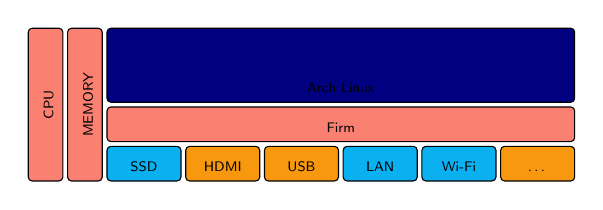
\begin{tikzpicture}[anchor=base,font=\tiny]
    \node at ($(\grdnxa, 0)
      + 0.5*(0, \grdclya + \grdclyc + \grdclw)$) [rotate=90] {CPU};
    \node at ($(\grdnxb, 0)
      + 0.5*(0, \grdclya + \grdclyc + \grdclw)$) [rotate=90] {MEMORY};

    \node at (\grdnxc, \grdnya) {SSD};
    \node at (\grdnxd, \grdnya) {HDMI};
    \node at (\grdnxe, \grdnya) {USB};
    \node at (\grdnxf, \grdnya) {LAN};
    \node at (\grdnxg, \grdnya) {Wi-Fi};
    \node at (\grdnxh, \grdnya) {\ldots};
    \node at ($(0.5*(\grdclxc + \grdclxh + \grdclw, 0)
      + (0, \grdnyb)$) {Firm};
    \node at ($(0.5*(\grdclxc + \grdclxh + \grdclw, 0)
      + (0, \grdnyc)$) {Arch Linux};
 
    \begin{scope}[on background layer]
      \pgfsetcornersarced{\pgfpoint{0.05cm}{0.05cm}}
      \color{Salmon}
      \rectaabe
      \pgfusepath{fill}
      \rectbace
      \pgfusepath{fill}
      \color{ProcessBlue}
      \rectcadb
      \pgfusepath{fill}
      \color{YellowOrange}
      \rectdaeb
      \pgfusepath{fill}
      \recteafb
      \pgfusepath{fill}
      {
        \color{ProcessBlue} 
        \rectfagb
        \pgfusepath{fill}
        \rectgahb
        \pgfusepath{fill}
      }
      \recthaib
      \pgfusepath{fill}
      \color{Salmon}
      \rectcbic
      \pgfusepath{fill}
      \color{NavyBlue}
      \rectccie
      \pgfusepath{fill}

      \color{black}
      \rectaabe
      \pgfusepath{stroke}
      \rectbace
      \pgfusepath{stroke}
      \rectcadb
      \pgfusepath{stroke}
      \rectdaeb
      \pgfusepath{stroke}
      \recteafb
      \pgfusepath{stroke}
      \rectfagb
      \pgfusepath{stroke}
      \rectgahb
      \pgfusepath{stroke}
      \recthaib
      \pgfusepath{stroke}
      \rectcbic
      \pgfusepath{stroke}
      \rectccie
      \pgfusepath{stroke}
    \end{scope}
  \end{tikzpicture}

\end{document} 
% vi: se ts=2 sw=2 et:
